\section{Vandhøns (vildtkending og biologi)}

% ========== TITEL: VANDHØNS ==========
\begin{frame}
  \vspace{1.5em}
  \begin{center}
    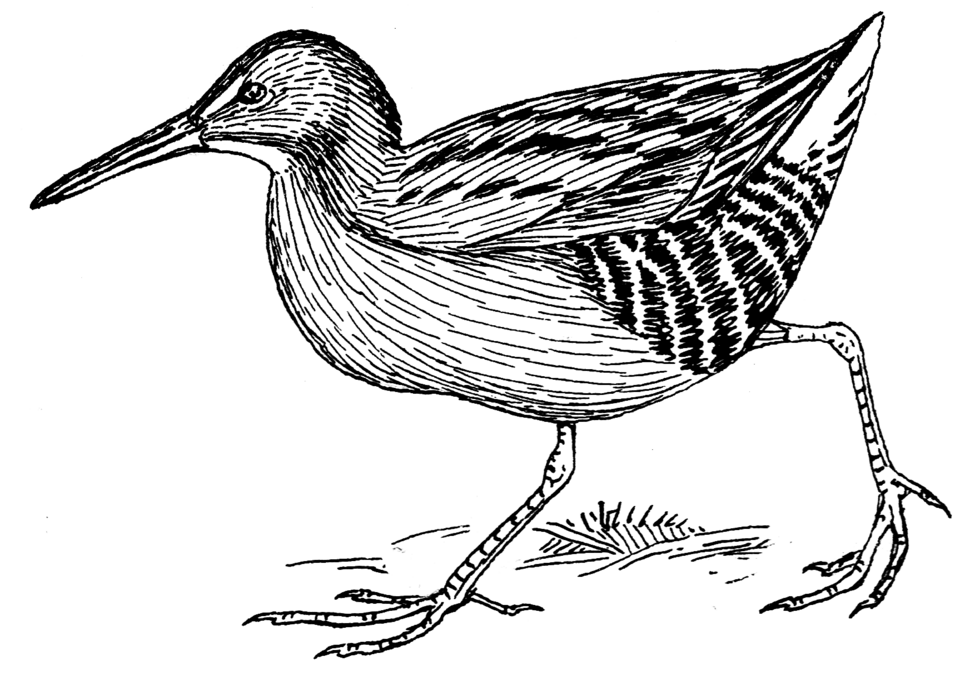
\includegraphics[width=12cm, height=4cm, keepaspectratio]{Billeder/Dyr/Fugle/Vandhøns/vandhøns.png}\\[1.2em]
    {\LARGE \textbf{Vandhøns}}\\[0.6em]
   
    Artsbestemmelse \& vildtbiologi\\[0.9em]
    {\tiny\color{gray}
    CC BY 4.0 – kan frit anvendes, også kommercielt. Rettighederne må ikke skærpes.\\[0.05em]
    Udviklet af Aleksander Sønder, OSJAGTTEGN.DK}
  \end{center}
\end{frame}

% ========== BLISHØNE ==========
\begin{frame}{%
  \begin{minipage}[c]{0.30\textwidth}
    Blishøne
  \end{minipage}%
  \hfill
  \begin{minipage}[c]{0.45\textwidth}
    \footnotesize
    \textbf{Jagttid:} 1.\ oktober -- 31.\ januar
  \end{minipage}%
  \hfill
  \begin{minipage}[c]{0.15\textwidth}
    \noindent\raggedleft
    
\includegraphics[width=0.5cm, height=0.5cm, keepaspectratio]{Billeder/Ikoner/star.png}%
    \hspace{0.2em}%
    
\includegraphics[width=0.5cm, height=0.5cm, keepaspectratio]{Billeder/Ikoner/star.png}
  \end{minipage}%
}
  \vspace{0.25em}
  \begin{columns}[T]
    \column{0.45\textwidth}
    \setlength{\parskip}{0.5em}
    \tiny
    \RaggedRight
    \textbf{\textit{Fulica atra}} – kraftig vandfugl med rund, skifersort krop og lange ben \par
    \textbf{Udseende:}\\
    \quad – Sort fjerdragt \\
    \quad – Hvid pandeblis \\
    \quad – Næb med rosa spids \par
    \textbf{Levesteder:} Søer og indre farvande. \par
    \textbf{Føde:} Vandplanter suppleret med muslinger, insekter og bløddyr. \par
    \textbf{Udbredelse:} Hele Danmark. \par
    \textbf{Træk/standfugl:} Begge
    \column{0.52\textwidth}
    \centering
    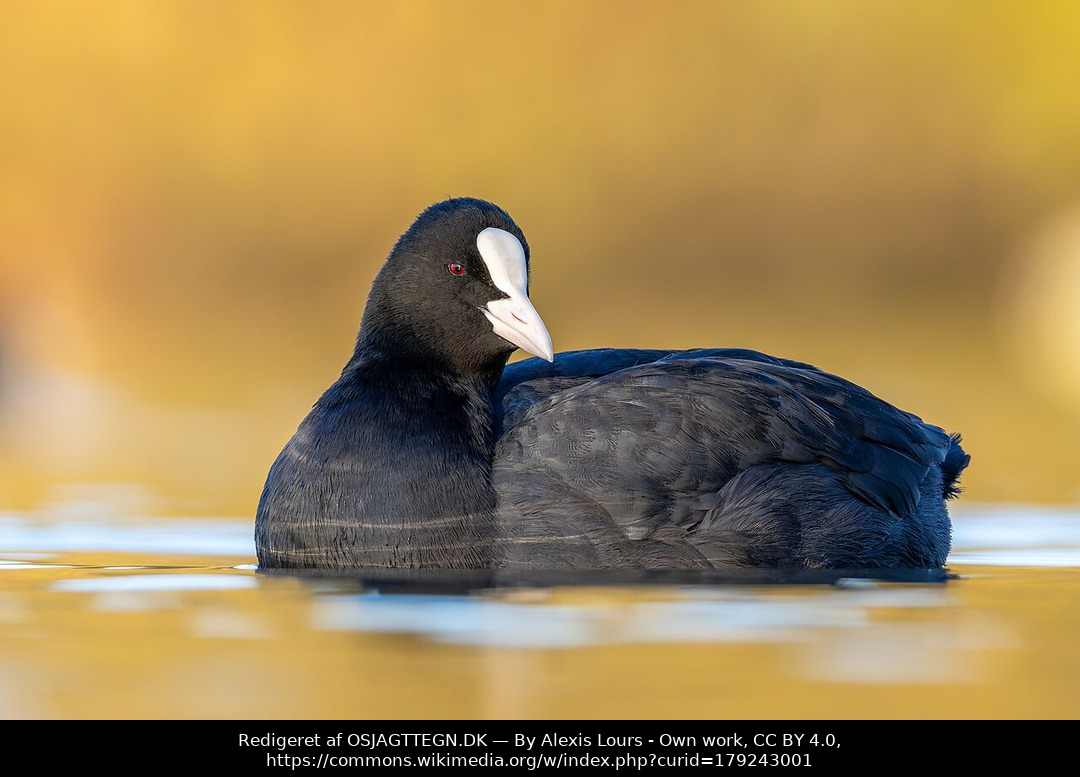
\includegraphics[width=\linewidth, height=7.2cm, keepaspectratio]{Billeder/Dyr/Fugle/Vandhøns/blishoene-01.jpg}
  \end{columns}
\end{frame}
% ========== GRØNBENET RØRHØNE ==========
\begin{frame}{%
  \begin{minipage}[c]{0.30\textwidth}
    Grønbenet rørhøne
  \end{minipage}%
  \hfill
  \begin{minipage}[c]{0.45\textwidth}
    \footnotesize
    \textbf{Jagttid:} Ingen jagttid
  \end{minipage}%
  \hfill
  \begin{minipage}[c]{0.15\textwidth}
    \noindent\raggedleft
    
\includegraphics[width=0.5cm, height=0.5cm, keepaspectratio]{Billeder/Ikoner/star.png}
  \end{minipage}%
}
  \vspace{0.25em}
  \begin{columns}[T]
    \column{0.45\textwidth}
    \setlength{\parskip}{0.5em}
    \tiny
    \RaggedRight
    \textbf{\textit{Gallinula chloropus}} – slankere end blishønen \par
    \textbf{Udseende:}\\
    \quad – Sort med hvid flankestribe \\
    \quad – Rødt næb med gul spids \\
    \quad – Rødt pandeskjold og grønlige ben
    \column{0.52\textwidth}
    \centering
    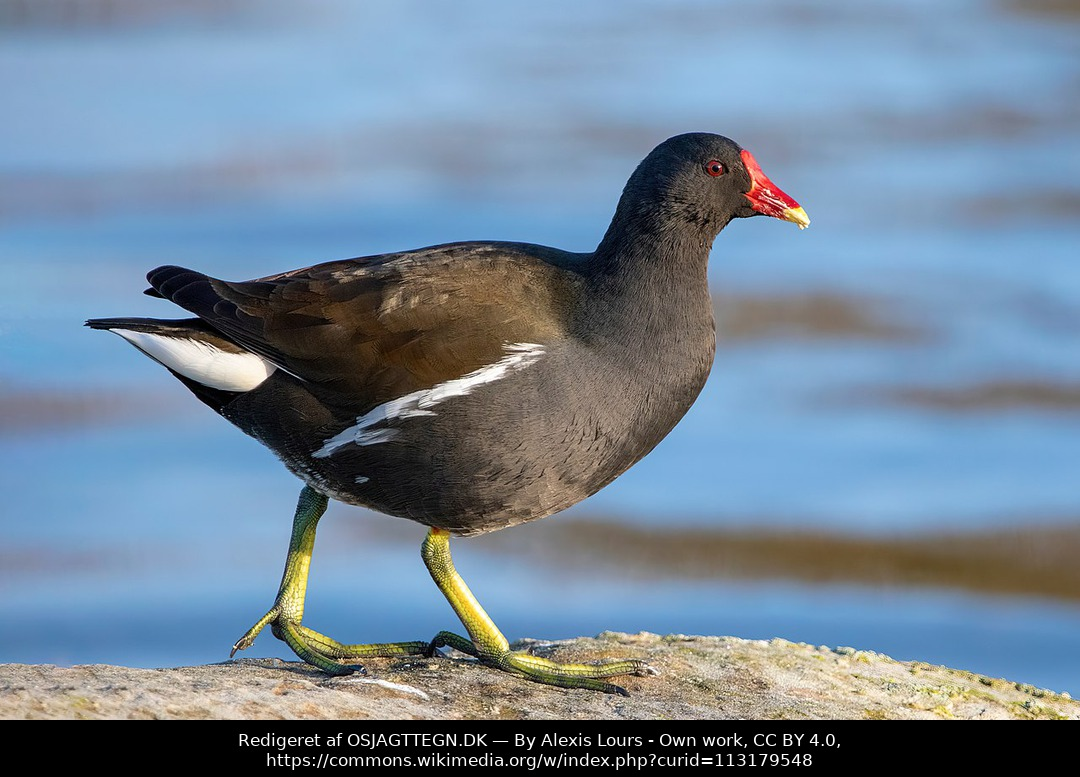
\includegraphics[width=\linewidth, height=7.2cm, keepaspectratio]{Billeder/Dyr/Fugle/Vandhøns/groenbenetroerhoene-02.jpg}
  \end{columns}
\end{frame}
\begin{frame}
  \vspace{1.8em}
  \begin{center}
    \begin{minipage}{0.22\textwidth}
      \centering
      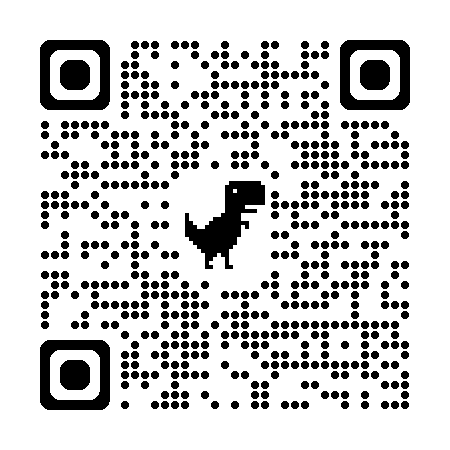
\includegraphics[width=\linewidth]{Billeder/Dyr/Fugle/Vandhøns/qr/vandhøns_qr.png}
    \end{minipage}%
    \hspace{0.8em}%
    \begin{minipage}{0.62\textwidth}
      \raggedright
      \Large
      \textbf{Træning i artsbestemmelse af vandhøns}\\[0.35em]
      {\large https://osjagttegn.dk/vandhoens}
    \end{minipage}
  \end{center}
\end{frame}